\chapter{A função Delta de Dirac e a propriedade da convolução}
\section{A função Delta de Dirac}
Muitos fenômenos físicos exigem a representação de uma força muito grande em um intervalo de tempo muito pequeno, por exemplo:
\begin{itemize}
 \item um circuito elétrico recebe uma força eletromotriz grande em um curto intervalo de tempo.
 \item um sistema massa-mola é atingido por uma martelo.
 \item uma bola de futebol parada recebe um chute, ou seja, uma força quase instantânea, que a coloca em movimento.
 \item um avião é atingido por um raio.
\end{itemize}
Para representar essa força, vamos tomar a função pulso unitário em um curto intervalo de tempo $[-\epsilon,\epsilon]$ em torno da origem, isto é, um pulso com integral unitária:
\begin{equation}
\delta_\epsilon(t)=\frac{1}{2\epsilon}\left(u(t+\epsilon)-u(t-\epsilon)\right)=\left\{\begin{array}{ll}0,&t<-\epsilon\\ \frac{1}{2\epsilon},&-\epsilon<t<\epsilon\\0,&t>\epsilon.\end{array}\right.
\end{equation}
Um pulso unitário em torno de $t=a$ é representado por
\begin{equation}{\label{def_delta_dirac}}
\delta_\epsilon(t-a)=\frac{1}{2\epsilon}\left(u(t-(a-\epsilon))-u(t-(a+\epsilon))\right)=\left\{\begin{array}{ll}0,&t<a-\epsilon\\ \frac{1}{2\epsilon},&a-\epsilon<t<a+\epsilon\\0,&t>a+\epsilon.\end{array}\right.
\end{equation}
Observe que $\int_{-\infty}^\infty\delta_\epsilon(t-a)=1$ para qualquer $\epsilon>0$. A figura \ref{fig_delta_dirac} apresenta o gráfico de $\delta_\epsilon(t-a)$ para $a>0$ e $\epsilon=1$, $\epsilon=\frac{1}{2}$, $\epsilon=\frac{1}{4}$, $\epsilon=\frac{1}{8}$ e $\epsilon=\frac{1}{12}$.
A função que representa uma grande força instantânea é chamada de {\bf função impulso} ou {\bf função Delta de Dirac} e pode ser definida pelo limite das funções pulsos:
\begin{equation}
\delta(t-a)=\lim_{\epsilon\to 0}\delta_\epsilon(t-a).
\end{equation}
Este limite não pode ser interpretado pontualmente, isto é, como o limite usual de funções reais, mas apenas no contexto de uma integral, como veremos.
A figura \ref{fig_delta_dirac} apresenta o gráfico de $\delta_\epsilon(t-a)$ quando $\epsilon$ diminui e uma representação gráfica para $\delta(t-a)$.
\begin{figure}[!ht]
\begin{center}

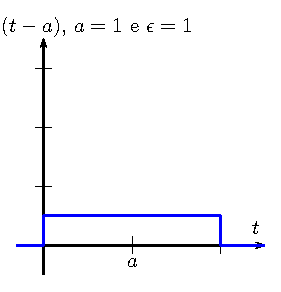
\includegraphics{cap_dirac_conv/pics/figura_1}\hspace{20pt}
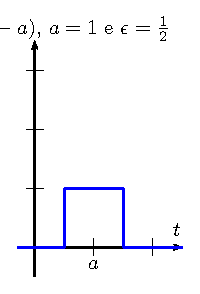
\includegraphics{cap_dirac_conv/pics/figura_2}\hspace{20pt}
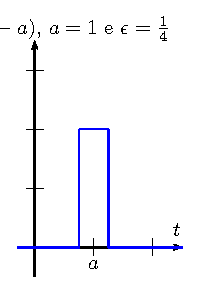
\includegraphics{cap_dirac_conv/pics/figura_3}

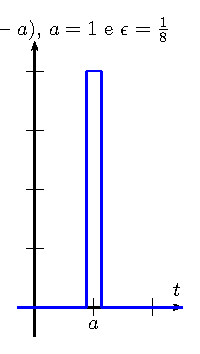
\includegraphics{cap_dirac_conv/pics/figura_4}\hspace{20pt}
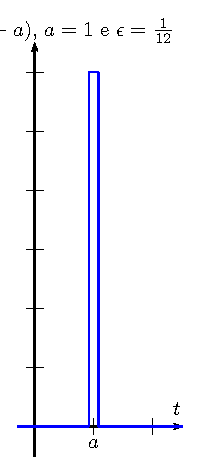
\includegraphics{cap_dirac_conv/pics/figura_5}\hspace{20pt}
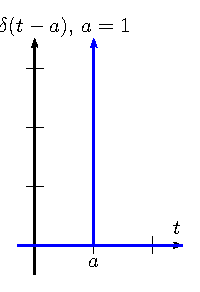
\includegraphics{cap_dirac_conv/pics/figura_6}
\end{center}
\caption{\label{fig_delta_dirac}}
\end{figure}
\begin{obs}A função delta de Dirac pode ser definida como limite de outras sequências de funções com propriedades análogas a sequência de pulsos. Por exemplo, podemos definir $\delta(t)$ como limite das funções
\begin{equation}
f_\epsilon(t)=\frac{1}{\epsilon\sqrt{\pi}}e^{-\frac{t^2}{\epsilon^2}}
\end{equation}
\end{obs}
A função Impulso é zero em todo ponto, exceto em $t=a$:
\begin{equation}
\delta(t-a)=\left\{\begin{array}{ll}0,&t\neq a\\\infty,&t=a  \end{array}\right.
\end{equation}
e
\begin{equation}
\int_{-\infty}^\infty\delta(t-a)dt=1
\end{equation}
A função Delta de Dirac deve ser sempre compreendida como o limite de funções reais no contexto de uma integração, isto conduz à chamada  {\bf propriedade da filtragem}, que define totalmente a Delta da Dirac:
Se $f(t)$ for um função contínua em torno de $t=a$, então
\begin{equation}{\label{prop_filtragem_dirac}}
\int_{-\infty}^\infty \delta(t-a)f(t)dt=f(a). 
\end{equation}
Para chegar a esta conclusão, definimos $F(t)=\int_a^t f(\tau)d\tau$ e calculamos:
\begin{eqnarray*}
\int_{-\infty}^\infty \delta(t-a)f(t)dt&=&\lim_{\varepsilon\to 0+}
\int_{-\infty}^\infty \delta_\varepsilon(t-a)f(t)dt\\
&=&\frac{1}{2\varepsilon}\int_{-\varepsilon}^\varepsilon f(t)dt\\
&=&\frac{F(\varepsilon)-F(-\varepsilon)}{2\varepsilon}\\
&=&F'(0)=f(a).
\end{eqnarray*}
\subsection{Delta de Dirac como derivada distribucional da função Heaviside}
Na equação (\ref{def_delta_dirac}) definimos a função Delta de Dirac como
\begin{equation}
\delta(t-a)=\lim_{\epsilon\to 0}\frac{1}{2\epsilon}\left(u(t-(a-\epsilon))-u(t-(a+\epsilon))\right).
\end{equation}
Por outro lado, usamos a definição de derivada para escrever
\begin{equation}
\lim_{\epsilon\to 0}\frac{1}{2\epsilon}\left(u((t-a)+\epsilon))-u((t-a)-\epsilon))\right)=\frac{d}{dt}u(t-a)
\end{equation}
ou seja,
\begin{equation}
\delta(t-a)=\frac{d}{dt}u(t-a).
\end{equation}
Observe que as funções de Heaviside e de Dirac não são funções no sentido do cálculo diferencial e integral. Naturalmente, a derivada acima também vale somente num sentido generalizado, mas é coerente quando olhamos a função de Heaviside como limite de funções rampas (ver figura \ref{fig_Heaviside_1}), pois na origem a derivada tende ao infinito.
A transformada de Laplace de função Delta de Dirac é obtido pela propriedade da filtragem dada na equação (\ref{prop_filtragem_dirac}):
\begin{equation}{\label{prop_trans_delta_dirac}}
\mathcal{L}\{\delta(t-a)\}=\int_0^\infty \delta(t-a)e^{-st}dt=e^{-as}.
\end{equation}

\subsection*{Exercícios}%Delta

\begin{exer}
Encontre
\begin{itemize}
  \item[a)] $\displaystyle \mathcal{L} \big\{ t u(t-1) + t^2 \delta(t-1) \big\}$
  \item[b)] $\displaystyle \mathcal{L} \big\{ (\cos t) ( \ln t ) \delta(t-\pi) \big\}$
  \item[c)] $\displaystyle \mathcal{L}\left\{ \delta(t-1) e^t \right\}$
\end{itemize}
\end{exer}
\begin{resp}
\begin{itemize}
  \item[a)] $\displaystyle \frac{ e^{-s} (s^2 + s + 1) }{s^2}$
  \item[b)] $\displaystyle -e^{-\pi s} \ln \pi $
  \item[c)] $\displaystyle e^{1-s}$
  \end{itemize}
\end{resp}
\begin{exer}
Calcule a solução dos seguintes problemas de valor inicial:
\begin{itemize}
  \item[a)] $\displaystyle \left\{
                              \begin{array}{ll}
                                y'' + 2y'+2y = \delta(t-\pi)\\
                                y(0) = 1, \quad y'(0)=0
                              \end{array}
                            \right.
  $
  \item[b)] $\displaystyle \left\{
                              \begin{array}{ll}
                                y'' + 3y'+2y = \delta(t-5) - u(t-10)\\
                                y(0) = 0, \quad y'(0)=1/2
                                \end{array}
                            \right.
  $
  \item[c)] $\displaystyle \left\{
                              \begin{array}{ll}
                                y'' + y = \delta(t-2\pi)\\
                                y(0) = 0, \quad y'(0)=1
                              \end{array}
                            \right.
  $
  \item[d)] $ \displaystyle \left\{\begin{array}{l}
   y''-2y'=1+\delta(t-2)\\
   y(0)=0\\
   y'(0)=1
  \end{array}\right.
 $
  
\end{itemize}
\end{exer}
\begin{resp}
\begin{itemize}
  \item[a)] $\displaystyle y(t) = e^{-t} \sen t + e^\pi e^{-t} \sen (t-\pi) u (t-\pi)  + e^{-t} \cos t  = e^{-t} \sen t \big( 1 - e^\pi u (t-\pi) \big)  + e^{-t} \cos t$
  \item[b)] $\displaystyle y(t) = \frac{1}{2} ( e^{-t} - e^{-2t} ) +  ( e^{5-t} - e^{10-2t} )u(t-5) - \frac{1}{2} (1 - 2e^{10-t} + e^{20-2t} )u(t-10)$
  \item[c)] $\displaystyle y(t) = \sen t + \sen(t-2\pi) u(t-2\pi)$
\end{itemize}
\end{resp}
\begin{exer}{\label{ex_delta_dirac0}} Considere as funções $f_\varepsilon (t)$  e $g_\varepsilon (t)$ dadas por
\begin{eqnarray*}
 f_\varepsilon(t)&=&\left\{\begin{array}{ll}
			    \frac{t}{\varepsilon^2}, ~~ &0\leq t < \varepsilon\\~\\
			    \frac{2\varepsilon-t}{\varepsilon^2}, ~~ &\varepsilon\leq t < 2\varepsilon\\~\\
			    0,&t\geq 2\varepsilon
			    \end{array}
\right.\\~\\
g_\varepsilon(t)&=&\left\{\begin{array}{ll}
			    \frac{1}{\varepsilon^2}, ~~ &0\leq t < \varepsilon\\~\\
			    -\frac{1}{\varepsilon^2}, ~~ &\varepsilon< t < 2\varepsilon\\~\\
			    0,&t>2\varepsilon
			    \end{array}
\right.
\end{eqnarray*}
onde $\varepsilon$ é um parâmetro positivo.
\begin{itemize}
  \item [a)] Esboce sob o mesmo plano cartesiano o gráfico da função $f_\varepsilon$ para $\varepsilon=1$, $\varepsilon=\frac{1}{2}$ e $\varepsilon=\frac{1}{4}$. Faça o mesmo em outro plano cartesiano para a função $g_\varepsilon(t)$. Lembre de indicar os eixos e pontos notáveis (ex. pontos de zero e máximo)
  \item [b)] Calcule as transformada de Laplace, $F_\varepsilon(s)=\mathcal{L}\left\{f_\varepsilon(t)\right\}$ e $G_\varepsilon(s)=\mathcal{L}\left\{g_\varepsilon(t)\right\}$. Aqui $\varepsilon$ é um parâmetro positivo genérico.
\item [c)] Estude o comportamento das funções $f_\varepsilon(t)$, $g_\varepsilon(t)$, $F_\varepsilon(s)$ e $G_\varepsilon(s)$ no limite $\varepsilon\to 0+$. Discuta os resultados obtidos analisando as função no domínio tempo e no domínio frequência (s). Qual a relação que se observa entre $f_\varepsilon(t)$ e $g_\varepsilon(t)$ e entre suas transformadas de Laplace?
\end{itemize}
\end{exer}


\section{Aplicação: circuito RLC}{\label{sec_circ_2}}
Considere o circuito Resistor/Capacitor/Indutor representado na figura \ref{fig_circ_2} com uma tensão $V(t)$ aplicada do tipo pulso,
\begin{equation}
V(t)=V_0\left(u(t-a)-u(t-b)\right).
\end{equation}
\begin{figure}[!ht]
\begin{center}

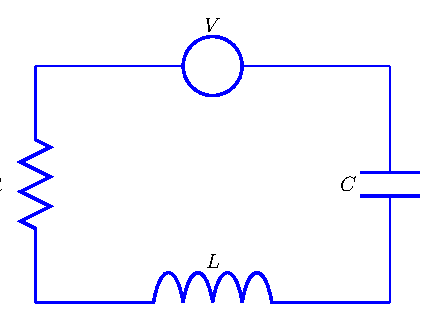
\includegraphics{cap_dirac_conv/pics/figura_7}\end{center}
\caption{\label{fig_circ_2}}
\end{figure} 
O modelo para a corrente $i(t)$ obedece a lei de Kirchoff:
\begin{equation}{\label{modelo_corrente}}
Li'(t)+ Ri(t)+\frac{1}{C}q(t)=V_0\left(u(t-a)-u(t-b)\right),
\end{equation}
onde $q(t)$ é a carga no capacitor, $\frac{1}{C}q(t)$ é a tensão no capacitor de capacitância $C$, $Ri(t)$ é a tensão no resistor de resistência $R$ e $Li'(t)$ é a tensão no indutor de indutância $L$. Considere as condições iniciais $i(0)=0$ e $q(0)=0$.
Dado que $\frac{dq(t)}{dt}=i(t)$, derivamos a equação (\ref{modelo_corrente}) para obter a seguinte equação diferencial:
\begin{equation}{\label{modelo_corrente_2}}
Li''(t)+ Ri'(t)+\frac{1}{C}i(t)=V_0\left(\delta(t-a)-\delta(t-b)\right),
\end{equation}
onde usamos que a derivada da função de Heaviside é a função delta de Dirac. As condições iniciais para a equação (\ref{modelo_corrente_2}) são $i'(0)=0$ e $i(0)=0$. Com o objetivo de resolver a problema de valor inicial, aplicamos a transformada de Laplace para obter a equação subsidiária
\begin{equation*}
Ls^2I(s)+ RsI(s)+\frac{1}{C}I(s)=V_0\left(e^{-as}-e^{-bs}\right),
\end{equation*}
que tem solução
\begin{eqnarray*}
I(s)&=&\frac{V_0\left(e^{-as}-e^{-bs}\right)}{Ls^2+Rs+\frac{1}{C}}\\
&=&\frac{1}{L}\frac{V_0\left(e^{-as}-e^{-bs}\right)}{\left(s+\frac{R}{2L}\right)^2-\left(\frac{R}{2L}\right)^2+\frac{1}{LC}}\\
&=&\frac{V_0}{L}\left[\frac{e^{-as}}{\left(s+\frac{R}{2L}\right)^2+\eta}-\frac{e^{-bs}}{\left(s+\frac{R}{2L}\right)^2+\eta}\right]
\end{eqnarray*}
onde
\begin{equation}
\eta=\frac{1}{LC}-\left(\frac{R}{2L}\right)^2.
\end{equation}
Vamos exemplificar os casos subamortecido, superamortecido e criticamente amortecido tomando $V_0=10V$, $a=1$ e $b=5$:
\begin{itemize}
 \item Caso subamortecido ($\eta>0$): escolhemos o caso onde $L=1\ \!$H, $C=\frac{1}{10}\ \!$F e $R=2\Omega$. Nesse caso
 \begin{equation}
 I(s)=10\left[\frac{e^{-s}}{\left(s+1\right)^2+9}-\frac{e^{-5s}}{\left(s+1\right)^2+9}\right].
 \end{equation}
 Logo,
 \begin{equation}
 i(t)=\frac{10}{3}\left(u(t-1)e^{-(t-1)}\sen\left(3 (t-1)\right)-u(t-5) e^{-(t-5)}\sen\left(3 (t-5)\right)\right).
 \end{equation}
 O gráfico da corrente é apresentado na figura \ref{fig_circ_RCL_1}.
\begin{figure}[!ht]
\begin{center}

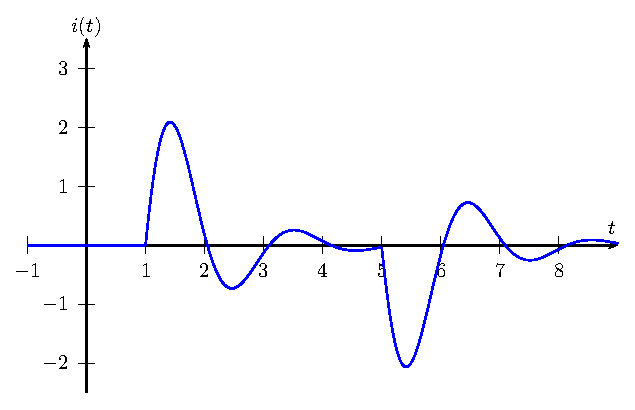
\includegraphics{cap_dirac_conv/pics/figura_8}\end{center}
\caption{\label{fig_circ_RCL_1}}
\end{figure}
 \item Caso superamortecido ($\eta<0$): escolhemos o caso onde $L=1\ \!$H, $C=1\ \!$F e $R=4\Omega$. Nesse caso
 \begin{equation}
 I(s)=10\left[\frac{e^{-s}}{\left(s+2\right)^2-3 }-\frac{e^{-5s}}{\left(s+2\right)^2-3}\right].
 \end{equation}
 Logo,
 \begin{eqnarray*}
 i(t)&=&10\left(u(t-1)\frac{e^{-2(t-1)}}{ \sqrt{3}}\senh\left(\sqrt{3} (t-1)\right)-u(t-5)\frac{e^{-2(t-5)}}{\sqrt{3} }\senh\left(\sqrt{3}  (t-5)\right)\right)\\
 &=&\frac{5}{\sqrt{3}}u(t-1)\left(e^{\left(\sqrt{3}-2\right) (t-1)}-e^{-\left(\sqrt{3}+2\right) (t-1)}\right)+\\
 &+&\frac{5}{\sqrt{3}}u(t-5)\left(e^{\left(\sqrt{3}-2\right) (t-5)}-e^{-\left(\sqrt{3}+2\right) (t-5)}\right)
 \end{eqnarray*}
 O gráfico da corrente é apresentado na figura \ref{fig_circ_RCL_2}.
\begin{figure}[!ht]
\begin{center}

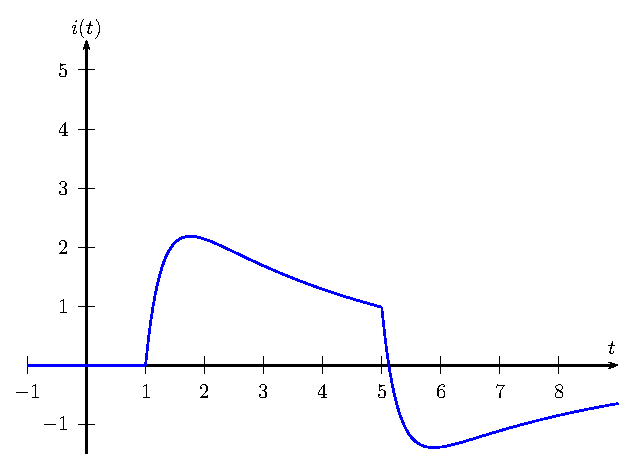
\includegraphics{cap_dirac_conv/pics/figura_9}\end{center}
\caption{\label{fig_circ_RCL_2}}
\end{figure}
\item Caso criticamente amortecido ($\eta=0$): escolhemos o caso onde $L=1\ \!$H, $C=1\ \!$F e $R=2\Omega$. Nesse caso
 \begin{equation}
 I(s)=10\left[\frac{e^{-s}}{\left(s+1\right)^2}-\frac{e^{-5s}}{\left(s+1\right)^2}\right].
 \end{equation}
 Logo,
 \begin{equation}
 i(t)=10\left(u(t-1)e^{-(t-1)} (t-1)-u(t-5)e^{-(t-5)} (t-5)\right).
 \end{equation}
O gráfico da corrente é apresentado na figura \ref{fig_circ_RCL_3}.
\begin{figure}[!ht]
\begin{center}

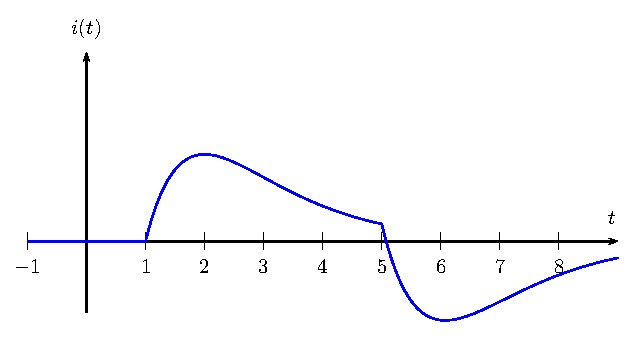
\includegraphics{cap_dirac_conv/pics/figura_10}\end{center}
\caption{\label{fig_circ_RCL_3}}
\end{figure}
\end{itemize}

\subsection*{Exercícios}
\begin{exer}
Um capacitor de capacitância $C$ está inicialmente carregado de forma que seu potencial seja $V_0$. A partir de $t=0$, o capacitor se descarrega através de um resistor de resistência $R$ (veja figura \ref{circ_1}). Use o método da transformada de Laplace para encontrar a carga $q(t)$ no capacitor.
\begin{figure}[!ht]
\begin{center}

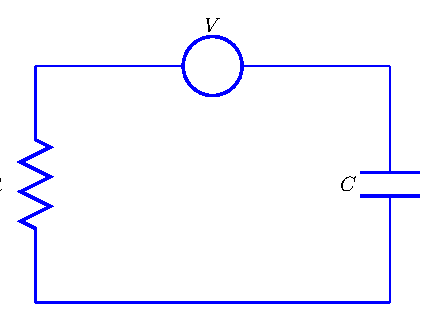
\includegraphics{cap_dirac_conv/pics/figura_14}\end{center}
\caption{\label{circ_1}}
\end{figure}
\end{exer}
\begin{resp}
 $\displaystyle q(t) = C V_0 e^{-t/RC}$
\end{resp}
\begin{exer}
Dado o circuito LC da figura \ref{circ_2}, encontre a corrente $i(t)$ e faça seu gráfico, assumindo $L = 1$ H, $C = 1$ F, corrente inicial nula, carga inicial no capacitor nula e $V(t) = u(t) - u(t-a)$.
\begin{figure}[!ht]
\begin{center}

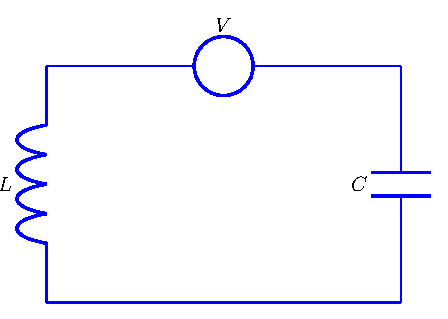
\includegraphics{cap_dirac_conv/pics/figura_15}\end{center}
\caption{\label{circ_2}}
\end{figure}
\end{exer}
\begin{resp}
 $\displaystyle i(t) = \sen t - \sen(t-a) u(t-a)$
\end{resp}
\begin{exer}
Dado o circuito RLC da figura \ref{circ_3}, encontre a corrente $i(t)$, assumindo que a corrente e a carga iniciais sejam nulas e que $R= 2 \ \Omega$, $L = 1$ H, $C = 1/2$ F e 
\begin{equation}
V(t) = \left\{
                                               \begin{array}{ll}
                                                 1, & \hbox{se } t\in (0,2) \\
                                                 0, & \hbox{se } t>2
                                               \end{array}
                                             \right.
\end{equation}
\begin{figure}[!ht]
\begin{center}

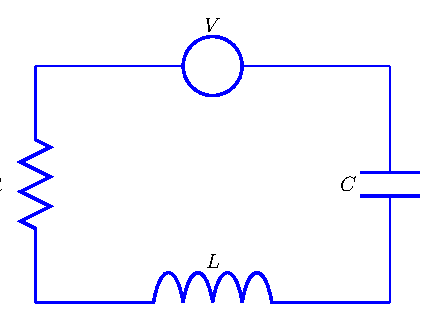
\includegraphics{cap_dirac_conv/pics/figura_16}\end{center}
\caption{\label{circ_3}}
\end{figure} 
\end{exer}
\begin{resp}
 $\displaystyle i(t) = e^{-t}\sen t - u(t-2)  e^{2-t} \sen (t-2)$
\end{resp}
\begin{exer}
Dada a equação do movimento de um oscilador harmônico simples (OHS)
\begin{equation}\label{ohs}
-k y(t) - \gamma y'(t) + f = my''(t),
\end{equation}
calcule a resposta $y(t)$ deste oscilador sujeito a forças externas $f$ do tipo dado abaixo. Considere $m=1$, $k=2$, $\gamma =3$, $y(0)=0$ e $y'(0)=0$.
\begin{itemize}
  \item[a)] $\displaystyle f(t) = \left\{
                                         \begin{array}{ll}
                                           1, & \hbox{ se } t\in [1,2] \\
                                           0, & \hbox{caso contrário}
                                         \end{array}
                                       \right.
  $
  \item[b)] $\displaystyle f(t) = \delta (t-1)$
\end{itemize}
\end{exer}
\begin{resp}
\begin{itemize}
\item[a)] $\displaystyle y(t) = \frac{1}{2}\big[ 1 -2 e^{1-t} + e^{2-2t} \big]u(t-1) - \frac{1}{2}\big[ 1 - 2 e^{2-t} + e^{4 - 2t} \big]$
  \item[b)] $\displaystyle y(t) = \big[ e^{1-t} - e^{2-2t}\big] u(t-1)$
\end{itemize}
\end{resp}
\begin{exer}
Considere um OHS não amortecido, isto é, $\gamma = 0$ na equação diferencial associada \eqref{ohs}. Suponha que este oscilador está sujeito a uma força externa dada por $f = F_0 \sen \left( \sqrt{k/m} t\right)$.
\begin{itemize}
  \item[a)] Use o método da transformada de Laplace para calcular as oscilações forçadas $y(t)$, sabendo que $y(0) = 0$ e $y'(0)=0$.
  \item[b)] Como se comporta o gráfico destas oscilações? Que fenômeno físico você identifica?
\end{itemize}
\end{exer}
\begin{resp}
 $\displaystyle \frac{F_0}{2k} \big[ \sen(\sqrt{k/m}t) - \sqrt{k/m}t \cos(\sqrt{k/m}t) \big] $
\end{resp}

\begin{exer}
A equação do movimento de um OHS não amortecido sujeito a oscilações forçadas pode ser escrita como
\begin{equation}
y''(t) + \omega^2 y(t) = r(t), \quad \hbox{ onde } \ \omega= \sqrt{\frac{k}{m}} \ \hbox{ e } \ r(t) = \frac{f(t)}{m}.
\end{equation}
\begin{itemize}
  \item[a)] Pelo método da transformada de Laplace, encontre $Y(s) = \mathcal{L} \left\{y(t)\right\}$.
  \item[b)] Com o auxílio do Teorema da Convolução, encontre $y(t)$ (em termos de $R = \mathcal{L}\{r\}$).
\end{itemize}
\end{exer}
\begin{resp}
\begin{itemize}
   \item[a)] $\displaystyle F(s) = \frac{sy(0)+y'(0)}{s^2 + w^2} + \frac{R(s)}{s^2 + w^2}$
  \item[b)] $\displaystyle y(t) = y(0) \cos (\omega t) + \frac{y'(0) \sen (\omega t)}{\omega} + \frac{\sen (\omega t)}{\omega} \ast r(t)$
\end{itemize}
\end{resp}



\section{Aplicação: cálculo da deflexão em vigas sujeitas a cargas concentradas}
Considere uma viga elástica horizontal de comprimento $L$ sob a ação de forças verticais. Colocamos o eixo horizontal $x$ com origem no extremo a esquerda da viga e, portanto, $x=L$ é o outro extremo. Supomos que a viga está sujeita a uma carga $W(x)$ que provoca uma deflexão em cada ponto $x\in[0,L]$. Então, para pequenas deflexões podemos aproximar a curvatura $k(x)$ pela variação instantânea de $\theta(x)$, onde $\theta(x)$ é o ângulo entre o eixo $x$ e a tangente, ou seja, 
\begin{equation}{\label{def_viga01}}
k(x)=\frac{d\theta(x)}{dx}.
\end{equation}
Como
\begin{equation}
\frac{dy(x)}{dx}=\tan(\theta(x))
\end{equation}
e, para $\theta(x)$ pequeno, $\tan(\theta(x))\approx \theta(x)$, temos:
\begin{equation}{\label{def_viga02}}
\frac{dy(x)}{dx}=\theta(x),
\end{equation}
Derivamos a equação (\ref{def_viga02}) e substituímos na equação (\ref{def_viga01}) para obter
\begin{equation}{\label{def_viga03}}
\frac{d^2y(x)}{dx^2}=k(x).
\end{equation}
Por outro lado, a lei de Hooke para materiais nos dá $k(x)=\frac{M(x)}{EI}$, onde $E$ é o módulo de Young, $I$ é o momento de inércia da viga e $M(x)$ é o momento fletor. Assim, substituindo na equação (\ref{def_viga03}),
\begin{equation}{\label{def_viga04}}
\frac{d^2y(x)}{dx^2}=\frac{M(x)}{EI}.
\end{equation}
A variação do momento de inércia $M(x)$ é a força de cisalamento $V(x)$:
\begin{equation}
\frac{d}{dx}M(x)=V(x)
\end{equation}
e a variação da força de cisalamento é a carga:
\begin{equation}
\frac{d}{dx}V(x)=W(x).
\end{equation}
Logo,
\begin{equation}{\label{def_viga05}}
\frac{d^2}{dx^2}M(x)=W(x).
\end{equation}
Derivamos a equação (\ref{def_viga04}) duas vezes e substituímos na equação (\ref{def_viga05}) para obter a equação de Euler-Bernoulli:
\begin{equation}
\label{eq}\frac{d^4}{dx^4}y(x)=\frac{1}{EI}W(x).
\end{equation}
Consideraremos aqui uma viga engastada, ou seja: \begin{equation}y(0)=y'(0)=y(L)=y'(L)=0.\end{equation}
A carga está concentrada na posição $x=\frac{L}{3}$ e tem intensidade $P_0$, sendo modelada pela seguinte expressão:
\begin{equation}W(x)=P_0\delta\left(x-\frac{L}{3}\right).\end{equation}
Aplicando a transformada de Laplace em (\ref{eq}) e usando o fato que $\mathcal{L}\left(\delta\left(x-\frac{L}{3}\right)\right)=e^{-\frac{L}{3}s}$, obtemos
\begin{equation}s^4Y(s)-s^3y(0)-s^2y'(0)-sy''(0)-y'''(0)=\frac{P_0}{EI}e^{-\frac{L}{3}s}\end{equation}
Substituimos $y(0)=y'(0)=0$, $y''(0)=C_1$ e $y'''(0)=C_2$ onde $C_1$ e $C_2$ são constantes a determinar:
\begin{equation}s^4Y(s)-sC_1-C_2=\frac{P_0}{EI}e^{-\frac{L}{3}s}\end{equation}
finalmente:
\begin{equation}Y(s)=\frac{C_1}{s^3}+\frac{C_2}{s^4}+\frac{P_0}{EI}\frac{e^{-\frac{L}{3}s}}{s^4}\end{equation}
e recuperamos a solução do domínio $x$ através da transformada inversa de Laplace:
\begin{equation}y(x)=\frac{C_1}{2!}x^2+\frac{C_2}{3!}x^3+\frac{P_0}{EI}\frac{(x-L/3)^3}{3!}u(x-L/3).\end{equation}
A expressão para $y(x)$ pode ser escrita como função definida por partes na forma:
\begin{equation}y(x)=\left\{\begin{array}{ll}\frac{C_1}{2!}x^2+\frac{C_2}{3!}x^3,&0\leq x\leq\frac{L}{3} \\ \frac{C_1}{2!}x^2+\frac{C_2}{3!}x^3+\frac{P_0}{EI}\frac{(x-L/3)^3}{3!},&\frac{L}{3}<x\leq L .\end{array}\right.\end{equation}
Para calcular o valor das constantes $C_1$ e $C_2$ calculamos  $y(L)$ e $y'(L)$ usando a segunda parte da função $y(x)$:
\begin{eqnarray*}
0=y(L)&=&\frac{C_1}{2}L^2+\frac{C_2}{6}L^3+\frac{4}{81}\frac{P_0}{EI}L^3\\
0=y'(L)&=&C_1 L+\frac{C_2}{2}L^2+\frac{2}{9}\frac{P_0}{EI}L^2
\end{eqnarray*}
Colocando na forma matricial:
\begin{equation}\left[\begin{array}{cc}
\frac{L^2}{2} & \frac{L^3}{6}\\
L & \frac{L^2}{2}\\
\end{array}
\right]\left[\begin{array}{c}
C_1\\
C_2\end{array}
\right]=\left[\begin{array}{c}
-\frac{4}{81}\frac{P_0}{EI}L^3\\
-\frac{2}{9}\frac{P_0}{EI}L^2\end{array}.
\right]
\end{equation}
 Invertemos a matriz do sistema para obter as constantes $C_1$ e $C_2$:
\begin{equation}\left[\begin{array}{c}
C_1\\
C_2\end{array}
\right]=
\frac{12}{L^4}
\left[\begin{array}{cc}
\frac{L^2}{2} & -\frac{L^3}{6}\\
-L & \frac{L^2}{2}\\
\end{array}
\right]\left[\begin{array}{c}
-\frac{4}{81}\frac{P_0}{EI}L^3\\
-\frac{2}{9}\frac{P_0}{EI}L^2\end{array}
\right],
\end{equation}
o que resulta em $C_1=\frac{4P_0 L}{27EI}$ e $C_2=-\frac{20P_0 }{27EI}$. A figura \ref{viga} apresenta o gráfico da função $y(x)$ quando $L=5$ e $\frac{P_0}{EI}=1$.
\begin{figure}[!ht]
\begin{center}

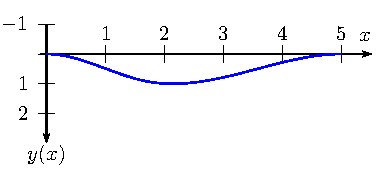
\includegraphics{cap_dirac_conv/pics/figura_11}\end{center}
\caption{\label{viga}}
\end{figure}

%\subsection*{Exercícios}


\section{Aplicação: metabolismo de uma medicação}
Durante um período de consumo de uma medicação, a concentração da substância ingerida na corrente sanguinea evolui segundo um modelo simples da seguinte forma:
\begin{itemize}
 \item No caso de ausência de dosagens, a variação da concentração é proporcional a concentração.
 \item  O organismo metaboliza o medicamento com uma taxa $\tau$.
  \item As doses de medicamento são liberadas e entra na corrente sanguinea instantaneamente e homogeneamente.
\end{itemize}
O modelo que descreve esse fenômeno é
\begin{equation}
c'(t)+\frac{1}{\tau}c(t)=x(t),\qquad t>0
\end{equation}
onde $c(t)$ é a concentração e $x(t)$ representa a dosagem ao longo do tempo $t$. Em geral, as dosagens não são únicas e são tomadas periodicamente. Seja $c_0$ a concentração administrada instantaneamente a cada período $T$, então
\begin{equation}
x(t)=c_0\left(\delta(t)+\delta(t-T)+\delta(t-2T)+\delta(t-3T)+\cdots\right)
\end{equation}
Supondo que $c(0)=0$, ou seja, inicialmente não havia substância no organismo, vamos calcular $c(t)$. 
Começamos aplicando a transformada de Laplace:
\begin{equation}
sC(s)+\frac{1}{\tau}C(s)=c_0\left(1+e^{-sT}+e^{-2sT}+e^{-3sT}+\cdots\right)=c_0\sum_{n=0}^\infty\left( e^{-sT}\right)^n.
\end{equation}
e encontramos:
\begin{equation}
C(s)=\left(\frac{c_0}{ s+\frac{1}{\tau}}\right)\sum_{n=0}^\infty\left( e^{-sT}\right)^n.
\end{equation}
Calculamos a transformada inversa usando a propriedade do deslocamento no eixo $s$.
\begin{eqnarray*}
c(t)&=&c_0\left(e^{-\frac{t}{\tau}}+e^{-\frac{t-T}{\tau}}u(t-T)+e^{-\frac{t-2T}{\tau}}u(t-2T)+e^{-\frac{t-3T}{\tau}}u(t-3T)+\cdots\right) \\
&=&c_0e^{-\frac{t}{\tau}}\left(1+e^{\frac{T}{\tau}}u(t-T)+e^{\frac{2T}{\tau}}u(t-2T)+e^{\frac{3T}{\tau}}u(t-3T)+\cdots\right)
\end{eqnarray*}
 O gráfico da concentração é apresentado na figura \ref{concentracao}, usando $c_0=1$, $\tau=1$ e $T=1$.
\begin{figure}[!ht]
\begin{center}

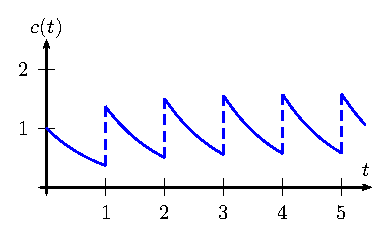
\includegraphics{cap_dirac_conv/pics/figura_12}\end{center}
\caption{\label{concentracao}}
\end{figure}
O salto em cada descontinuidade é exatamente $c_0$, pois os limites laterais são
\begin{eqnarray*}
\lim_{t\to nT^-}c(t)&=&\lim_{t\to nT^-}\left(c_0e^{-\frac{t}{\tau}}\left(1+e^{\frac{T}{\tau}}+e^{\frac{2T}{\tau}}+\cdots+ e^{\frac{(n-1)T}{\tau}}\right)\right)\\
&=&\left(c_0e^{-\frac{nT}{\tau}}\left(1+e^{\frac{T}{\tau}}+e^{\frac{2T}{\tau}}+\cdots+ e^{\frac{(n-1)T}{\tau}}\right)\right)\\
&=&\left(c_0\left(e^{-\frac{nT}{\tau}}+e^{-\frac{(n-1)T}{\tau}}+e^{-\frac{(n-2)T}{\tau}}+\cdots+ e^{-\frac{T}{\tau}}\right)\right)\\
\end{eqnarray*}
e
\begin{eqnarray*}
\lim_{t\to nT^+}c(t)&=&\lim_{t\to nT^+}\left(c_0e^{-\frac{t}{\tau}}\left(1+e^{\frac{T}{\tau}}+e^{\frac{2T}{\tau}}+\cdots+ e^{\frac{(n-1)T}{\tau}}+ e^{\frac{nT}{\tau}}\right)\right)\\
&=&\left(c_0e^{-\frac{nT}{\tau}}\left(1+e^{\frac{T}{\tau}}+e^{\frac{2T}{\tau}}+\cdots+ e^{\frac{(n-1)T}{\tau}}+ e^{\frac{nT}{\tau}}\right)\right)\\
&=&\left(c_0\left(e^{-\frac{nT}{\tau}}+e^{-\frac{(n-1)T}{\tau}}+e^{-\frac{(n-2)T}{\tau}}+\cdots+ e^{-\frac{T}{\tau}}+1\right)\right),\\
\end{eqnarray*}
que possuem diferença igual a $c_0$. 
Observe que quando calculamos o limite $\displaystyle \lim_{t\to 0^+}c(t)$ obtemos $c(0^+)=c_0$, valor diferente da condição inicial dada, que é $c(0)=0$. Apesar de parecer estranho, não está errado. Tudo é consequência da presença do Dirac em $t=0$, que produz uma discontinuidade na origem. Este assunto será discutido na seção \ref{problemas_na_origem}.



\section{Problemas na origem}\label{problemas_na_origem}
Para entender melhor esse fenômeno, vamos considerar um problema um pouco mais simples, dado pelo seguinte problema de valor inicial:
\begin{equation*}
\left\{
\begin{array}{rcl}
y'(t)+y(t)&=&\delta(t)\\
y(0)&=&0
\end{array}
\right.
\end{equation*}
Tomando a Transformada de Laplace, temos:
\begin{equation*}
sY(s)-y(0)+Y(s)=1
\end{equation*}
ou seja, $Y(s)=\frac{1}{s+1}$, o que implica
\begin{equation}y(t)=e^{-t}.\end{equation}
Observamos que $y(0)=1\neq 0$, ou seja, a condição inicial não é satisfeita.
Para entendermos o que está acontecendo, devemos lembrar que a Transformada de Laplace só produz a solução para $t>0$ e interpretar $y(t)$ como
\begin{equation}y(t)=u(t)e^{-t}.\end{equation}
Desta forma $y(0)$ simplesmente não está definido. De fato, para compreender esse comportamento, vamos definir um problema auxiliar colocando no lugar da função delta de Dirac uma função pulso:
\begin{equation*}
\left\{
\begin{array}{rcl}
y'(t)+y(t)&=&\frac{u(t)-u(t-\varepsilon)}{\varepsilon}\\
y(0)&=&0
\end{array}
\right.
\end{equation*}
onde $\varepsilon$ é uma constante positiva pequena. Sabemos que o termo \begin{equation}\frac{u(t)-u(t-\varepsilon)}{\varepsilon}\end{equation} converge para $\delta(t)$ quando $\varepsilon \to 0+$. Aplicando a Transformada de Laplace e resolvendo para $Y(s)$, temos:
\begin{equation}Y(s)=\frac{1}{s(s+1)}\frac{1-e^{-\varepsilon s}}{\varepsilon}=\left(\frac{1}{s}-\frac{1}{s+1}\right)\frac{1-e^{-\varepsilon s}}{\varepsilon},\end{equation}
ou seja,
\begin{equation}y(t)=\frac{1-e^{-t}}{\varepsilon}u(t)-u(t-\varepsilon)\frac{1-e^{-(t-\varepsilon)}}{\varepsilon}.\end{equation}
Esta solução pode ser escrita como uma função contínua:
\begin{equation}y(t)=\left\{\begin{array}{ll}
0,&t\leq 0,\\~\\
\frac{1-e^{-t}}{\varepsilon},&0<t\leq \varepsilon,\\~\\
\frac{e^{\varepsilon}-1}{\varepsilon}~\!
e^{-t},&t\geq \varepsilon.
\end{array}
\right.\end{equation}
Para $\varepsilon>0$ pequeno podemos usar a seguinte aproximação:
\begin{equation}e^t=1+t+\frac{t^2}{2}+\frac{t^3}{3!}+\ldots \approx 1+t\end{equation}
Assim, temos:
\begin{equation}y(t)\approx\left\{\begin{array}{ll}
0,&t\leq 0,\\~\\
\frac{t}{\varepsilon},&0<t\leq \varepsilon,\\~\\
e^{-t},&t\geq \varepsilon.
\end{array}
\right.\end{equation}
Ou seja, existe uma pequena região de transição entre $0$ e $\varepsilon$ onde a solução $y(t)$ sobe rapidamente. O gráfico apresentado na figura \ref{concentracao_2} mostra o comportamento de $y(t)$ para $\varepsilon=0.2$, $\varepsilon=0.1$ e $\varepsilon=0.05$ em azul, vermelho e verde, respectivamente, assim como a solução limite $e^{-t}u(t)$ em preto.
\begin{figure}[!ht]
\begin{center}

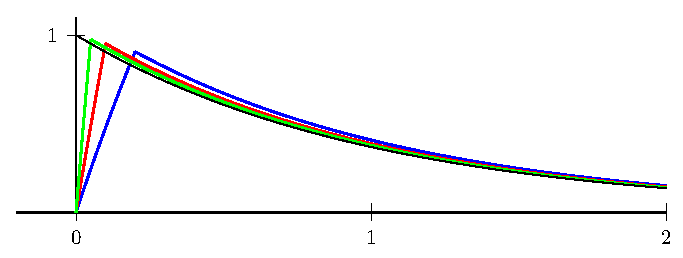
\includegraphics{cap_dirac_conv/pics/figura_13} \end{center}
\caption{\label{concentracao_2}}
 \end{figure}
 
 \subsection*{Exercícios}
\begin{exer}
Considere o seguinte problema de valor inicial:
 \begin{eqnarray*}
x'(t)&=&- x(t) -2 y(t)+\delta(t)\\
y'(t)&=& x(t) - y(t)+\delta(t),
\end{eqnarray*}
com $x(0)=0$ e $y(0)=0$.\\
 \indent  {a)}  Aplique o método de transformada de Laplace e escreva $X(s)=\mathcal{L}\{x(t)\}$ e $Y(s)=\mathcal{L}\{y(t)\}$ nos espaços abaixo.
 
\indent  {b)}  Calcule as transformadas inversas e escreva $x(t)$ e $y(t)$ abaixo.

\indent  {c)} Aplique sua solução do item b) nas condições inciais e justifique o resultado encontrado.\\

\end{exer}


\section{Propriedade da convolução}
Dada duas funções contínuas por partes em $[0,\infty]$, a convolução  de $f$ e $g$ denotada por $f*g$ é definida pela integral
\begin{equation}{\label{def_conv}}
 (f*g)(t)=\int_0^t f(\tau)g(t-\tau)d\tau.
\end{equation}
\begin{ex}{\label{ex_conv_1}}Dadas $f(t)=e^t$ e $g(t)=\cos(t)$, vamos calcular $f*g$:
\begin{eqnarray*}
 (f*g)(t)&=&\int_0^t e^{\tau} \cos(t-\tau)d\tau\\
 &=&\left. \frac{1}{2}e^\tau\left(\cos(t-\tau)-\sen(t-\tau)  \right)\right|_0^t\\
 &=& \frac{1}{2}\left(e^t-\cos(t)+\sen(t)  \right).
\end{eqnarray*}
onde usamos que $\int  e^{\tau} \cos(t-\tau)d\tau=\frac{1}{2}e^\tau\left(\cos(t-\tau)-\sen(t-\tau)  \right)+\ \!$constante.
\end{ex}
\begin{teo}{\label{prop_conv}}(Propriedade da convolução) Se $F(s)=\mathcal{L}\{f(t)\}$ e $G(s)=\mathcal{L}\{g(t)\}$, então
\begin{equation}{\label{eq_prop_conv}}
 \mathcal{L}\{(f*g)(t)\}=F(s)G(s).
\end{equation}
ou
\begin{equation}{\label{eq_inv_prop_conv}}
 \mathcal{L}^{-1}\{F(s)G(s)\}=(f*g)(t).
\end{equation}
\end{teo}
\begin{proof}Partimos da definição das transformadas:
\begin{equation}
F(s)=\mathcal{L}\{f(t) \}=\int_0^\infty f(t)e^{-st}dt
\end{equation}
e
\begin{equation}
G(s)=\mathcal{L}\{g(\tau) \}=\int_0^\infty g(\tau)e^{-s\tau}d\tau.
\end{equation}
Logo,
\begin{eqnarray*}
 F(s)G(s)&=&\int_0^\infty f(t)e^{-st}dt\int_0^\infty g(\tau)e^{-s\tau}d\tau\\
&=&\int_0^\infty f(t) \int_0^\infty g(\tau)e^{-s(t+\tau)} d\tau dt\\
\end{eqnarray*}
Mantemos $t$ fixo e fazemos a mudança de variável $v=t+\tau$ para obter:
\begin{eqnarray*}
 F(s)G(s)=\int_0^\infty f(t) \int_t^\infty g(v-t)e^{-sv}dv dt\\
\end{eqnarray*}
Agora, vamos mudar a ordem de integração na região que é a metade inferior do primeiro quadrante: em vez de variar $v$ em $[t,\infty]$ depois $t$ em $[0,\infty]$, primeiro vamos variar $t$ em $[0,v]$, depois $v$ em $[0,\infty]$, ou seja,
\begin{eqnarray*}
 F(s)G(s)&=&\int_0^\infty  \int_0^v f(t) g(v-t)e^{-sv} dt dv\\
 &=&\int_0^\infty \left( \int_0^v f(t) g(v-t)dt\right)e^{-sv}  dv\\
 &=&\int_0^\infty (f*g)e^{-sv}  dv\\
   &=&\mathcal{L}\{f*g\}
\end{eqnarray*}
\end{proof}
\begin{ex}Vamos calcular a transformada inversa de $\frac{s}{(s-1)(s^2+1)}$. Primeiro observamos que a expressão pode ser escrita como um produto de duas funções tabelas:
\begin{equation}
\frac{s}{(s-1)(s^2+1)}=\frac{1}{s-1}\frac{s}{s^2+1},
\end{equation}
 onde $\mathcal{L}^{-1}\left\{\frac{1}{s-1}\right\}=e^t$ e $\mathcal{L}^{-1}\left\{\frac{s}{s^2+1}\right\}=\cos(t)$. Usando a propriedade \ref{prop_conv} da convolução, temos
 \begin{equation}
 \mathcal{L}^{-1}\left\{\frac{1}{s-1}\frac{s}{s^2+1}\right\}=\int_0^t e^\tau \cos(t-\tau)d\tau.
 \end{equation}
 A convolução acima foi calculada no exemplo \ref{ex_conv_1}, logo
\begin{equation}
 \mathcal{L}^{-1}\left\{\frac{1}{s-1}\frac{s}{s^2+1}\right\}= \frac{1}{2}\left(e^t-\cos(t)+\sen(t)  \right).
 \end{equation}
 \end{ex}
 A propriedade \ref{prop_conv} da convolução pode ser útil para resolver equações integrais, como veremos no próximo exemplo.
 \begin{ex} Vamos resolver a seguinte equação integral:
 \begin{equation}
 y(t)=4+9\int_0^t y(\tau)(t-\tau)d\tau.
 \end{equation}
 Aplicamos a transformada de Laplace e usamos a propriedade \ref{prop_conv} da convolução com $f(t)=y(t)$ e $g(t)=t$ para obter:
 \begin{equation}
 \mathcal{L}\{y(t)\}=\frac{4}{s}+9\mathcal{L}\{y(t)\}\mathcal{L}\{t\}
 \end{equation}
 ou seja,
 \begin{equation}
 Y(s)=\frac{4}{s}+9Y(s)\frac{1}{s^2}.
 \end{equation}
 Logo,
 \begin{equation}
 Y(s)=\frac{s^2}{s^2-9}\frac{4}{s}=\frac{4s}{s^2-9}.
 \end{equation}
 Portanto,
 \begin{equation}
 y(t)=4\cosh(3t)
 \end{equation}
\end{ex}

\subsection*{Exercícios}%convolução
\begin{exer}
Encontre por integração:
\begin{itemize}
  \item[a)] $1\ast 1$
  \item[b)] $t \ast e^t $
  \item[c)] $1\ast \cos(\omega t)$
  \item[d)] $e^{kt}\ast e^{-kt}$
\end{itemize}
\end{exer}
\begin{resp}
\begin{itemize}
  \item[a)] $\displaystyle t$
  \item[b)] $\displaystyle e^{t} - t - 1$
  \item[c)] $\displaystyle \frac{1}{\omega}\sen (\omega t)$
  \item[d)] $\displaystyle \frac{1}{2k} (e^{kt} - e^{-kt}) = \frac{1}{k}\senh (k t)$
\end{itemize}
\end{resp}
\begin{exer}
Justifique as seguintes propriedades da operação de convolução:
\begin{itemize}
  \item[a)] $f\ast g = g \ast f$
  \item[b)] $(f\ast g)\ast h = f \ast (g \ast h)$
  \item[c)] $f\ast (g + h) = f\ast g + f\ast h$
  \item[d)] $(\delta\ast f)(t) = f(t)$
\end{itemize}
{\it [Dica: cuidado para não confundir as variáveis de integração que aparecerão no item (b).}
\end{exer}
\begin{resp}
\begin{itemize}
  \item[a)] 
  \begin{eqnarray*}
   f\ast g&=&\int_0^t f(\tau)g(t-\tau)d\tau\\
   &=&-\int_t^0 f(t-u)g(u)du\\
   &=&\int_0^t g(u)f(t-u)du\\
   &=&g\ast f
  \end{eqnarray*}
  \item[b)] 
    \begin{eqnarray*}
   (f\ast g)\ast h&=& \int_0^t \left(\int_0^\tau f(u) g(\tau-u) du \right) h(t-\tau) d\tau \\
   &=& \int_0^t \int_0^\tau f(u) g(\tau-u) h(t-\tau) du d\tau \\
   &=& \int_0^t \int_u^t f(u) g(\tau-u) h(t-\tau)  d\tau du \\
   &=& \int_0^t f(u) \int_u^t g(\tau-u) h(t-\tau)  d\tau du \\
   &=& \int_0^t f(u) \int_0^{t-u} g(v) h(t-u-v)  dv du \\
   &=& \int_0^t f(u) \left[(g\ast h)(t-u)\right]  du \\
   &=&f \ast (g \ast h)
  \end{eqnarray*}
  onde se fez a mudança $v=\tau-u$, $dv=d\tau$.
\end{itemize}
\end{resp}

\begin{exer}Resolva a seguinte equação integral:
\begin{equation}
y(t)=t+\int_0^t y(\tau)\sen(t-\tau)d\tau
\end{equation}
\end{exer}
\begin{exer}
Use o Teorema da Convolução para calcular \begin{equation}\mathcal{L}^{-1} \left( \frac{1}{(s+1)(s^2+1)} \right).\end{equation}
\end{exer}
\begin{resp}
 $\displaystyle \frac{1}{2} \big[ \sen t - \cos t + e^{-t} \big] $
\end{resp}
\begin{exer}
Use o Teorema da Convolução para resolver as seguintes equações integrais:
\begin{itemize}
  \item[a)] $\displaystyle y(t) = 1 + \int_0^t y(\tau) \ d\tau$
  \item[b)] $\displaystyle y(t) = 1 - \int_0^t y(\tau) (t-\tau) \ d\tau$
  \item[c)] $\displaystyle y(t) = te^{t} -2 e^t \int_0^t e^{-\tau} y(\tau) \ d\tau$
  \item[d)] $\displaystyle y(t) = 1 - \senh t + \int_0^t (1+ \tau )y(t- \tau) \ d\tau$
\end{itemize}
\end{exer}
\begin{resp}
\begin{itemize}
  \item[a)] $\displaystyle y(t) = e^{t}$
  \item[b)] $\displaystyle y(t) = \cos t$
  \item[c)] $\displaystyle y(t) = \senh t$
  \item[d)] $\displaystyle y(t) = \cosh t$
\end{itemize}
\end{resp}